\subsection{Results\label{sec:results}}

% \begin{table}[tb]
% \begin{center}
% \caption{Precision, recall and F1 of English-only models on the English TAC 2013 slot-filling task. LSTM+USchema ensemble outperforms any single model. \label{en-tac-table}}
% \begin{tabular}{|lrrr|}
% \hline
% \bf Model & \bf Recall & \bf Precision & \bf F1 \\
% \hline\hline
% CNN                 & 31.6 & 36.8 & 34.1 \\
% %CNN-parse           & ?	& ? & ? \\
% LSTM                & \bf 32.2 & 39.6 & 35.5  \\
% USchema             & 29.4 & \bf 42.6 & 34.8 \\
% \hline
% USchema+LSTM        & 34.4 & 41.9 & 37.7 \\
% USchema+LSTM+AN	& 36.7 & 43.1 & \bf 39.7 \\
% \hline
% \end{tabular}
% \end{center}
% \end{table}

% \begin{table}[tb]
% \begin{center}
% \caption{F1 scores of multilingual models on the English TAC 2013 slot-filling task. Jointly embedding English and Spanish entity pairs results in higher scores on the English evaluation. Our system uses no handwritten patterns and we are able to match \cite{roth2014relationfactory} and \cite{angeli2014stanford} both of which use hand written patterns. \label{en-es-tac-table}}
% \tabcolsep=0.15cm
% \begin{tabular}{|lrrr|}
% %\hspace{-10pt}
% \hline
% \bf Model & \bf En & \bf En+Es &\bf En+Es+dict\\
% \hline\hline
% CNN  & 34.1 & 34.0 & 33.9	\\
% LSTM & 35.5 & 35.2 & 35.8 \\
% USchema & 34.8 & 35.7  & --- \\
% \hline
% USchema+LSTM & 37.7 & 39.0 & 38.2 \\
% USchema+LSTM+AN & 39.7 & \bf 40.9  &  40.2 \\
% \hline
% \cite{roth2014relationfactory}* & 40.2 &--- & --- \\
% \cite{angeli2014stanford}* & 40.9 & --- & --- \\
% \hline
% \end{tabular}
% \end{center}
% \end{table}



\begin{table}[tb]
\begin{center}
\begin{tabular}{|lrrr|}
\hline
\bf Model & \bf Recall & \bf Precision & \bf F1 \\
\hline\hline
CNN                 & 31.6 & 36.8 & 34.1 \\
%CNN-parse           & ?	& ? & ? \\
LSTM                & 32.2 & 39.6 & \bf 35.5  \\
USchema             & 29.4 & 42.6 & 34.8 \\
\hline\hline
USchema+LSTM        & 34.4 & 41.9 & 37.7 \\
USchema+LSTM+Es        & 38.1 & 40.2 & \bf 39.2 \\
\hline\hline
USchema+LSTM+AN	& 36.7 & 43.1 & 39.7 \\
USchema+LSTM+Es+AN & 40.2 & 41.2 & \bf 40.7 \\
\citet{roth2014relationfactory} & 35.8 & 45.7 & 40.2 \\
%\hline\hline
%\citet{angeli2014stanford}* & --- & --- & 40.9 \\
%USchema+LSTM+Es+AN * &	43.1 & 41.2	& \bf 42.1 \\

\hline
\end{tabular}
\caption{Precision, recall and F1 of English-only models on the English TAC 2013 slot-filling task. AN refers to alternative names heuristic and Es referes to using additional spanish raw text at train time. LSTM+USchema ensemble outperforms any single model. Our system uses no handwritten patterns is able to out-perform all highly tuned competitive systems. \protect\citet{roth2014relationfactory} and \protect\citet{angeli2014stanford} %both use hand written patterns. * = optimal per relation tuning
\label{en-tac-table}}
\end{center}
\end{table}

\begin{table}[tb]
\begin{center}
\begin{tabular}{|lrrr|}
\hline
\bf Model & \bf Recall & \bf Prec. & \bf F1 \\
\hline\hline
CNN                 & 28.1 & 29.0 & 28.5 \\
%CNN-parse           & ?	& ? & ? \\
LSTM                & 27.3 & 32.9 & \bf 29.8  \\
USchema             & 24.3 & 35.5 & 28.8 \\
\hline\hline
USchema+LSTM        & 34.1 & 29.3 & 31.5 \\
USchema+LSTM+Es        & 34.4 & 31.0 & 32.6 \\
USchema+LSTM+AN        & 34.7 & 29.3 & 31.7 \\
USchema+LSTM+AN+Es        & 33.5 & 32.2 & \bf 32.8 \\
\hline\hline
\citet{angeli2014stanford} & 29.8 & 58.5 & 39.5 \\
RPI Blender & 29.4 & 47.8 & 36.4 \\
ICTAS\_OKN & 24.3 & 59.0 & 34.4 \\
UT Austin & 25.7 & 42.8 & 32.1 \\
\hline
\end{tabular}
\caption{Precision, recall and F1 of English-only models on the English TAC 2014 slot-filling task. Es referes to using additional spanish raw text at train time and AN is alternative names heuristic. We also show results for the top 4 performing systems in the official TAC 2014 scoring. Our system would rank 4/18 in the 2014 TAC Slot Filling competition behind systems that use both hand written patterns and active learning. Our system uses niether of these addtional annotations. -see  \protect\cite{SurdeanuMihai2014}. \label{2014-en-tac-table}}
\end{center}
\end{table}


%\begin{table}[tb]
%\begin{center}
%\caption{Precision, recall and F1 of English-only models on the English TAC 2012 slot-filling task. \label{2012-en-tac-table}}
%\begin{tabular}{|lrrr|}
%\hline
%\bf Model & \bf Recall & \bf Precision & \bf F1 \\
%\hline\hline
%CNN                 & 28.5 & 26.0 & 27.2 \\
%LSTM                & 26.9 & 27.1 & 27.0  \\
%USchema             & 22.0 & 34.2 & 26.8 \\
%\hline\hline
%USchema+LSTM        & 30.2 & 26.7 & 29.1 \\
%\citet{angeli2014stanford}* & --- & --- & 30.7 \\
%\hline
%\end{tabular}
%\end{center}
%\end{table}



\begin{table}[h!]

\begin{center}
\begin{tabular}{|lrr|}
\hline
\bf Model & \bf Es+En & \bf Es+En+dict  \\
\hline\hline
CNN 		                    & 11.4     & 13.8	\\
LSTM 	                        & 10.7     & 15.2   \\
USchema                         & 16.3     & --- \\
\hline
USchema+LSTM                    & 17.3     & \bf 20.0 \\
\hline
\end{tabular}
\caption{Zero-Annotation transfer learning F1 scores on 2012 Spanish TAC KBP slot-filling task. Adding a translation dictionary improves all encoder-based models. Ensembling LSTM and USchema models performs the best. \label{es-tac-table}}
\end{center}
\end{table}



%In experiments on the English and Spanish TAC KBC slot-filling tasks, we find that both USchema and LSTM models outperform the CNN across languages, and that USchema tends to perform slightly better than the LSTM as the only model. Ensembling the LSTM and USchema models further increases final F1 scores in all experiments, suggesting that the two different types of model compliment each other well. In Section \ref{sec:qual-anal} we present a qualitative analysis of our results which further confirms this hypothesis.

Table \ref{en-tac-table} presents the performance of our English models. First, observe that the LSTM substantially outperforms a CNN. Second, note that the LSTM achieves higher recall than USchema whereas USchema is more precision-biased. This confirms our hypothesis in Section~\ref{sec:non-comp} about the strengths and weaknesses of the two approaches. 
%US, which matches more short, non-compositional patterns, makes more precise predictions at the cost of an inability to predict when entities are connected by a pattern unseen during training. The LSTM can predict a relation using any text between entities observes at test time, gaining recall at the loss of precision. 
Unsurprisingly, ensembling the LSTM and USchema improves F1 by nearly 2 points over the strongest single model, USchema. Adding the alternative names (AN) technique described in Section \ref{sec:ds-el} increases F1 by an additional 2 points, resulting in an F1 score that is competitive with the state-of-the-art.

\todo{description of 2014 results}

In Tables \ref{en-tac-table} and \ref{2014-en-tac-table}, we demonstrate the effect of jointly learning English and Spanish models on English slot filling performance. Adding Spanish data improves our F1 scores by 1.5 points on 2013 and 1.1 on 2014 over using English alone.

\begin{figure}
\begin{center}
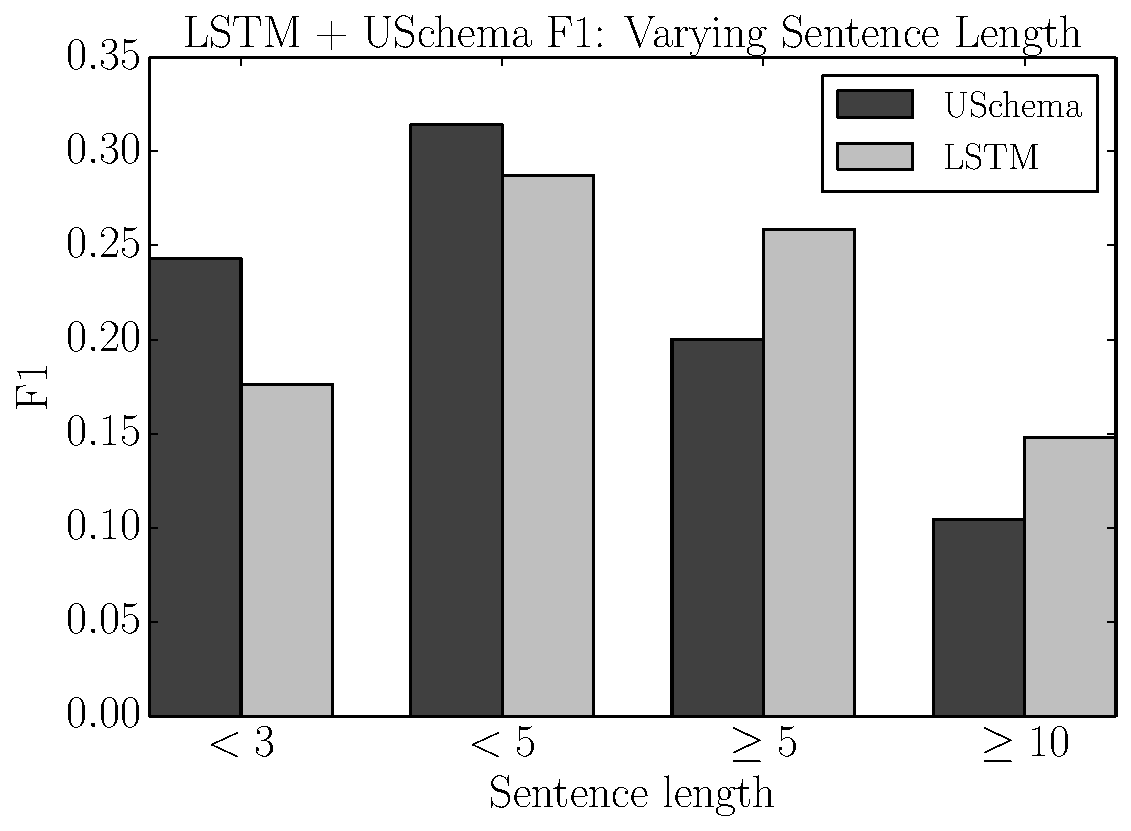
\includegraphics[scale=0.45]{f1-vary-sent-length}
\caption{F1 achieved by USchema vs. LSTM models for varying sentence lengths. LSTM performs better on longer sentences ($\geq$ 5 tokens) whereas USchema performs better on shorter sentences ($\leq 5$). \label{fig:f1-vary-sents}}
\end{center}
\end{figure}

Table \ref{es-tac-table} presents results for our Spanish relation extractors trained using zero-annotation transfer learning. For both the CNN and LSTM, tying word embeddings between the two languages results in substantial improvements. We see that ensembling the non-dictionary LSTM with USchema leads to a lower score than just USchema alone, but ensembling the dictionary-tied LSTM with USchema provides a significant increase of nearly 4 F1 points over the highest-scoring single model, USchema. Clearly, grounding the Spanish data using a translation dictionary provides much better Spanish word representations. These improvements are complementary to the baseline USchema model, and yield impressive results when ensembled. 


\subsection{Qualitative Analysis \label{sec:qual-anal}}

% error analysis
Analysis of our English models suggests that our encoder-based models (LSTM) extract relations based on a wide range of semantically similar patterns that the pattern-matching model (USchema) is unable to score due to a lack of exact string match in the test data. For example, Table \ref{tab:lstm-us-similar-rels} lists three examples of the \emph{per:children} relation that the LSTM finds which USchema does not, as well as three patterns that USchema does find. Though the LSTM patterns are all semantically and syntactically similar, they each contain different specific noun phrases, e.g. \emph{Lori}, \emph{four children}, \emph{toddler daughter}, \emph{Lee and Albert}, etc. Because these specific nouns weren't seen during training, USchema fails to find these patterns whereas the LSTM learns to ignore the specific nouns in favor of the overall pattern, that of a parent-child relationship in an obituary. USchema is limited to finding the relations represented by patterns observed during training, which limits the patterns matched at test-time to short and common patterns; all the USchema patterns matched at test time were similar to those listed in Table \ref{tab:lstm-us-similar-rels}: variants of \emph{'s son, '}. 


\begin{table}[h]
\begin{center}
\small
\begin{tabular}{|p{8cm}|}
\hline
\multicolumn{1}{|c|}{\textbf{LSTM}} \\ \hline
{\bf McGregor} \emph{is survived by his wife, Lori, and four children, daughters Jordan,} { \bf Taylor} and Landri, and a son, Logan. \\ \hline
In addition to his wife, {\bf Mays} \emph{is survived by a toddler daughter and a son,} {\bf Billy Mays Jr.}, who is in his 20s. \\ \hline
{\bf Anderson} \emph{is survived by his wife Carol, sons Lee and Albert, daughter} {\bf Shirley Englebrecht} and nine grandchildren. \\
\hline\hline
\multicolumn{1}{|c|}{\textbf{USchema}}  \\ \hline
{\bf Dio} \emph{'s son,} {\bf Dan Padavona}, cautioned the memorial crowd to be screened regularly by a doctor and take care of themselves, something he said his father did not do. \\ \hline
But {\bf Marshall} \emph{'s son,} {\bf Philip}, told a different story.  \\ \hline
``I'd rather have Sully doing this than some stranger, or some hotshot trying to
be the next Billy Mays,'' said the guy who actually is the next {\bf Billy Mays}\emph{, his son} {\bf Billy Mays III}. \\ 
\hline
\end{tabular}
\caption{Examples of the \emph{per:children} relation discovered by the LSTM and Universal Schema. Entities are bold and patterns italicized. The LSTM can model a richer set of patterns \label{tab:lstm-us-similar-rels}}
\end{center}
\end{table}

% cross lingual relations
Analysis of our multilingual models also suggests that they successfully embed semantically similar relations across languages using tied entity pairs and translation dictionary as grounding. Table \ref{tab:cross-lingual-relations} lists three top nearest neighbors in English for several Spanish patterns from the text. In each case, the English patterns capture the relation represented in the Spanish text. 

\newcommand{\tablespace}{\end{tabular}
\newline
\newline
%\hspace*{-21pt}
\begin{tabular}{|p{8cm}|}
}
\begin{table}[h]
\begin{center}
\small
%\hspace*{-21pt}
\begin{tabular}{|p{8cm}|}
\hline
\argOne y cuatro de sus familias, incluidos su esposa, Wu Shu-chen, su hijo, \argTwo\\
\it{\argOne and four of his family members, including his wife, Wu Shu-chen, his son, \argTwo} \\
\hline
\argOne and his son \argTwo \\
\argOne is survived by his wife, Sybil MacKenzie and a son, \argTwo \\
\argOne gave birth to a baby last week -- son \argTwo \\
\hline
\tablespace
\hline
\argOne (Puff Daddy, cuyos verdaderos nombre sea \argTwo \\
\it{\argOne (Puff Daddy, whose real name is \argTwo} \\
\hline%\hline
\argOne (usually credited as {\it E1} \\
\argOne (also known as Gero \#\#, real name \argTwo \\
\argOne and (after changing his name to \argTwo \\
\hline
\tablespace
%\hline
%\argOne, Tian Tian, de \#\# a\~{n}os de edad, y su madre \argTwo\\
%\it{\argOne, Tian Tian, \#\# years old, and his mother \argTwo} \\
%\hline%\hline
%\argOne Gyllenhaal's parents -- screenwriter Naomi Foner and director \argTwo \\
%\argOne Brando's mother, actress Anna Kashfi, divorced \argTwo \\
%\argOne Cash, his mom was \argTwo \\
%\hline
%\tablespace
\hline
\argOne lleg\'{o} a la alfombra roja en compa\~{n}\'{i}a de su esposa, la actriz Suzy Amis, casi una hora antes que su ex esposa, \argTwo\\
\it{\argOne arrived on the red carpet with his wife, actress Suzy Amis, nearly an hour before his ex-wife , \argTwo} \\
\hline%\hline
\argOne, who may or may not be having twins with husband \argTwo \\
\argOne, aged twenty, Kirk married \argTwo\\
\argOne went to elaborate lengths to keep his wedding to former supermodel \argTwo\\
\hline
%\tablespace
%\hline
%\bf{{\it E1} , una firmes of estudios económicos lleven sede in {\it E2}}\\
%\it{{\it E1} an economic studies firm with headquarters in {\it E2}} \\
%\hline\hline
%{\it E2} offices of BP and {\it E1} \\
%{\it E2} , the Paris - based {\it E1} \\
%{\it E2} province , is the headquarters of {\it E1} \\
%\hline
\end{tabular}
\caption{Top English patterns for a Spanish query pattern encoded using the dictionary LSTM: For each Spanish query (English translation in italics), a list of English nearest neighbors. \label{tab:cross-lingual-relations}}
\end{center}
\end{table}


In addition to embedding semantically similar phrases from English and Spanish to have high similarity, our models also learn high-quality multilingual word embeddings. In Table \ref{joint-word} we compare Spanish nearest neighbors of English query words learned by the LSTM with dictionary ties versus the LSTM with no ties, using no unsupervised pre-training for the embeddings. Both approaches jointly embed Spanish and English word types, using shared entity embeddings, but the dictionary-tied model learns qualitatively better multilingual embeddings. 


\begin{table}[h]
\setlength{\tabcolsep}{3pt}
\label{joint-word}
\small
\begin{center}
%\begin{minipage}[b]{0.45\linewidth}
%\hspace*{-17pt}
\begin{tabular}{|ll|}
\hline
\multicolumn{2}{|c|}{ \bf CEO}\\
\multicolumn{1}{|c}{Dictionary} & \multicolumn{1}{c|} {No Ties} \\ \hline 
jefe (chief)    & CEO \\ 
CEO & director (principle) \\
ejecutivo (executive)   &  directora (director) \\
cofundador (cofounder)  & firma (firm) \\
president (chairman) & magnate (tycoon)\\
\hline
%
\multicolumn{2}{|c|}{\bf headquartered}\\
\multicolumn{1}{|c}{Dictionary} & \multicolumn{1}{c|} {No Ties} \\ \hline
sede (headquarters) & Geol\'{o}gico (Geological) \\
situado (located) & Treki (Treki) \\
selectivo (selective) & Geof\'{i}sico(geophysical) \\
profesional (vocational) & Normand\'{i}a (Normandy)\\
bas\'{a}ndose (based) & emplea (uses)\\
\hline
%\end{tabular}
%\end{minipage}
%\hspace{-12.5pt}
%\begin{minipage}[b]{0.45\linewidth}
%\begin{tabular}{|ll|}
%\hline
\multicolumn{2}{|c|}{\bf hubby}\\
\multicolumn{1}{|c}{Dictionary} & \multicolumn{1}{c|} {No Ties} \\ \hline 
matrimonio (marriage)  & esposa (wife) \\ 
casada (married) & esposo (husband) \\
esposa (wife) &  casada(married) \\
cas\'{o} (married) & embarazada (pregnant)  \\
embarazada (pregnant) & embarazo (pregnancy) \\
\hline

%
\multicolumn{2}{|c|}{\bf alias}\\
\multicolumn{1}{|c}{Dictionary} & \multicolumn{1}{c|} {No Ties} \\ \hline
simplificado (simplified) & Weaver (Weaver)\\ 
sabido (known) & interrogaci\'{o}n (question) \\
seud\'{o}nimo (pseudonym)  &  alias \\
privatizaci\'{o}n (privatisation)  & reelecto (reelected) \\
nombre (name)  & conocido (known)\\
\hline
\end{tabular}
\caption{Example English query words (not in translation dictionary) in bold with their top nearest neighbors by cosine similarity listed for the dictionary and no ties LSTM variants. Dictionary-tied nearest neighbors are consistently more relevant to the query word than untied. }
%\end{minipage}
\end{center}
\end{table}




